\section{Introduction}
\label{sec:introduction}

Vehicle scheduling is a fundamental problem in intelligent transportation systems. It determines the order and timing with which vehicles from competing approaches pass a shared conflict area while maintaining safety and improving traffic efficiency. The same scheduling structure appears at signalized intersections, unsignalized intersections, freeway merging areas, work zones, roundabouts, and other locations where multiple traffic streams compete for a mutually exclusive spatial resource \citep{yu2017optimization,soleimaniamiri2020joint,rios2017automated,martingasulla2021traffic}. In connected and automated vehicle environments, vehicle-to-vehicle and vehicle-to-infrastructure communication further enables vehicles to negotiate conflict-free passing orders and trajectories in real time \citep{chen2016cooperative,li2006cooperative,liu2019trajectory}. Consequently, vehicle scheduling provides an important foundation for real-time traffic control and cooperative driving at general conflict areas.

Vehicle scheduling problems are often formulated as mixed-integer linear programs. In a vehicle-level formulation, each vehicle is represented by timing variables, while binary variables determine the relative order of vehicles from conflicting approaches. Safety constraints enforce the minimum following headway between vehicles from the same approach and the minimum switching headway between vehicles from different approaches. Such formulations can produce globally optimal schedules when solved to proven optimality. However, their computational burden grows rapidly with the number of vehicles because the number of pairwise ordering decisions increases approximately quadratically, while the corresponding branch-and-bound search can grow much faster \citep{chen2016cooperative,wolsey1999integer}. This scalability limitation is especially important in online control, where a central scheduler may have only a short time to return a usable solution.

Existing studies have addressed this difficulty through two broad classes of methods. The first class uses heuristic or approximate algorithms to construct feasible schedules with limited computational effort. Representative examples include conflict-point reservation methods, rule-based coordination, decentralized trajectory heuristics, and specialized merging or roundabout strategies \citep{debada2016autonomous,liu2019trajectory,rios2017automated,martingasulla2021traffic}. These methods can be effective in real-time applications, but they generally do not guarantee global optimality. The second class improves exact solution procedures through problem-specific search rules, decomposition, or tree pruning \citep{li2006cooperative,xu2019tree}. Such methods can reduce computation substantially for selected problem structures, but the underlying combinatorial difficulty remains as the number of vehicles increases.

Rather than developing another scheduling heuristic or solver enhancement, platoon-based scheduling addresses the problem structurally. Consecutive vehicles from the same approach are grouped into unified scheduling units before the downstream optimization problem is constructed \citep{bashiri2017platoon,xu2019grouping}. The scheduler then determines the order of platoons rather than the order of individual vehicles. This aggregation can sharply reduce the number of control units and pairwise ordering variables, thereby improving the tractability of the downstream mixed-integer program. However, requiring all vehicles within a platoon to pass consecutively also removes passing sequences in which vehicles from another approach are inserted inside that platoon. The reduced problem is therefore easier to solve, but its optimal objective value can be worse than that of the original vehicle-level problem.

This trade-off is not unique to vehicle scheduling. Aggregation is widely used to reduce the dimension of large optimization problems by replacing fine-grained decision units with coarser groups. Spatial aggregation merges demand regions in facility-location models \citep{daskin1989aggregation}; multilevel graph methods combine neighboring nodes before solving a reduced graph problem \citep{karypis1998fast,loukas2019graph}; and order batching groups customer orders to simplify warehouse routing and picking decisions \citep{cergibozan2019order}. Although these applications have different operational interpretations, they share the same basic tension: aggregation reduces computational burden by restricting the original solution space, and the restriction may cause a loss in solution quality. Figure~\ref{fig:platooning-tradeoff-concept} illustrates this trade-off by contrasting vehicle-level and platoon-level scheduling.

\begin{figure}[t]
  \centering
  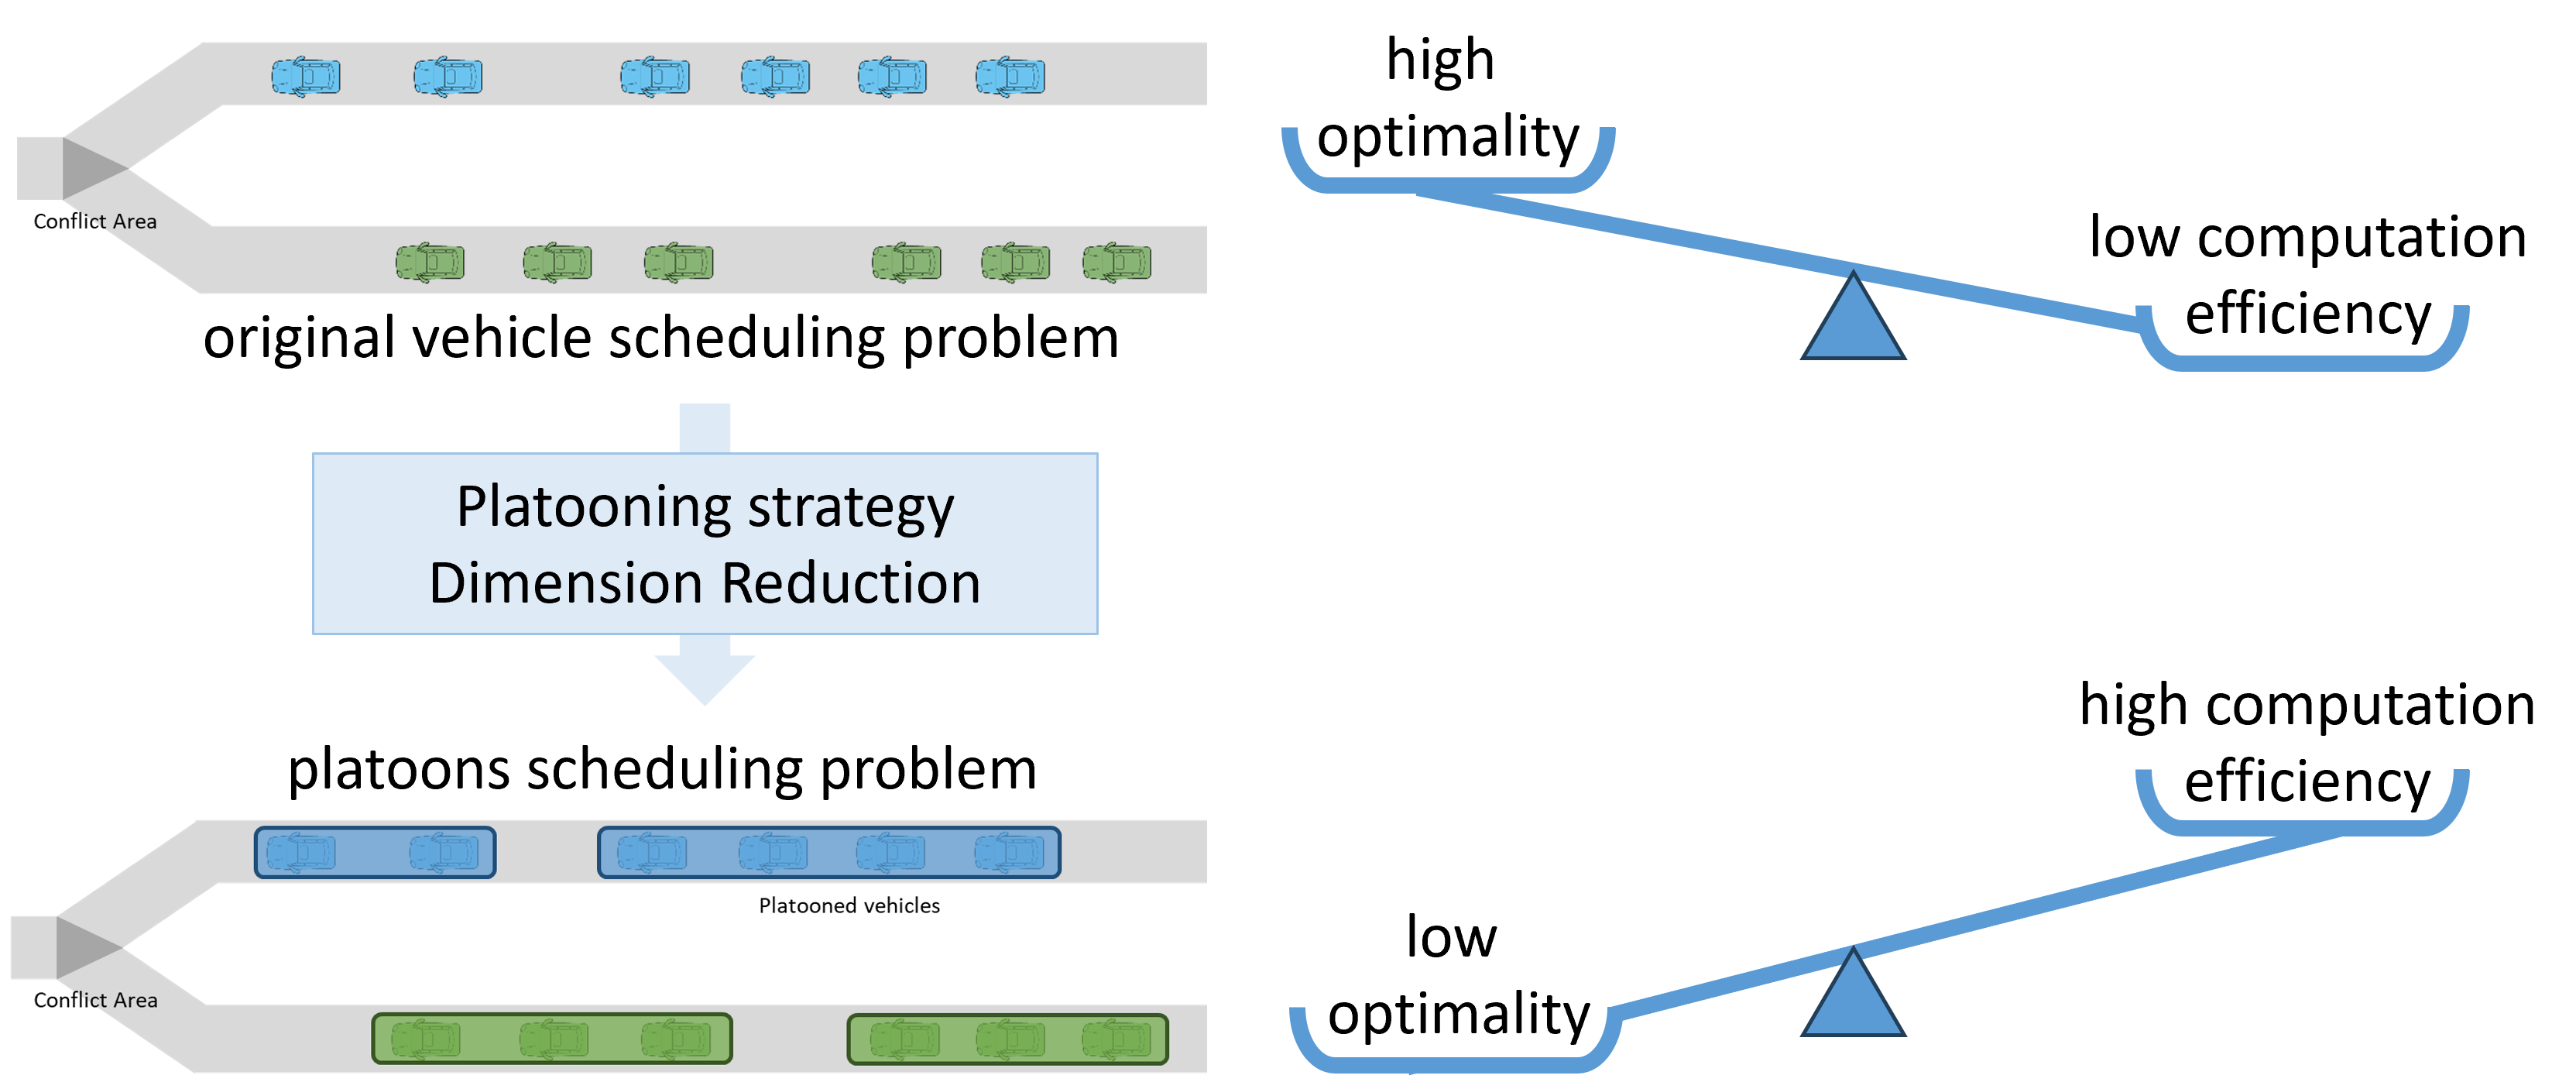
\includegraphics[width=0.95\linewidth]{figures/Picture1.png}
  \caption{Conceptual illustration of vehicle-level scheduling, platoon-level scheduling, and the resulting trade-off between scheduling flexibility and computational efficiency.}
  \label{fig:platooning-tradeoff-concept}
\end{figure}

Existing platoon-based vehicle-scheduling studies have demonstrated important computational benefits, but the performance loss caused by aggregation has mainly been evaluated numerically. The lack of theoretical analysis limits our understanding of how platooning parameters affect scheduling performance and makes parameter selection largely empirical. In particular, existing critical-headway platooning methods commonly group consecutive vehicles when their time gap is below a prescribed threshold, but they do not explicitly account for the effect of maximum platoon size on the resulting optimality gap.

This study analytically investigates the optimality--computation efficiency trade-off of platoon-based vehicle scheduling. We first characterize the optimality gap between vehicle-level scheduling and platoon-level scheduling and identify the factors that govern this gap. The analysis focuses on how the gap is affected by the headway between consecutive vehicles and by the number of vehicles grouped into a platoon. These theoretical insights are then incorporated into a simple rule-based platooning method that jointly considers a critical-headway threshold and a maximum platoon size. The proposed platoon-formation rule is deterministic, interpretable, and can be executed sequentially without solving an additional optimization problem.

The main contributions of this study are threefold:
\begin{enumerate}[label=(\roman*)]
  \item We derive an analytical upper bound on the scheduling optimality gap introduced by platooning and identify the key factors affecting this gap.
  \item We reveal the roles of the critical-headway threshold and maximum platoon size in controlling the trade-off between solution optimality and computation efficiency, and use these insights to design a simple rule-based platooning method.
  \item We evaluate the proposed method by comparing no platooning, conventional critical-headway platooning, and the proposed threshold-and-size platooning method in terms of scheduling performance and computational efficiency.
\end{enumerate}

The remainder of the paper is organized as follows. Section~\ref{sec:formulation} formulates the vehicle-level and platoon-constrained scheduling problems. Section~\ref{sec:theory} analyzes the platooning-induced optimality gap. Section~\ref{sec:dimension-reduction} presents the theory-guided rule-based platooning method. Section~\ref{sec:experiments} reports the numerical experiments. Section~\ref{sec:conclusion} concludes the paper.
